%-----------------------------------------------------------------------
\section{Extensions to Bayesian Optimization}

\begin{frame}{For what do we need extensions?}
\begin{block}{Standard BO Problem:}
\begin{itemize}
    \item Sequential optimization
    \pause
    \item Continuous, smooth functions
    \item Noise-free evaluations
    \item No constraints
\end{itemize}
\end{block}
\begin{block}{\emph{Exotic} BO Problem:}
\begin{itemize}
    \item Categorical hyperparameters
    \item Disconnected search spaces
    \item Parallel evaluations
    \item Noisy evaluations
    \item Optimization with constraints
    \item Multi-objective Bayesian optimization
\end{itemize}
\end{block}    
\end{frame}

%\begin{frame}[c]{Categorical and Conditional Parameters}
%\framesubtitle{Introduction}
%\begin{itemize}
%    \item<+->{Our parameter configuration space $\pcs$ can possibly contain:
%    \begin{itemize}
%        \item<+->{Neural Network Architectures.}
%        \item<+->{Model-specific parameters.}
%        \item<+->{General optimization parameters.} 
%    \end{itemize}
%    }
%    \item<+->{Consider searching through such a space of parameters. Is every individual dimension of this search space-
%    \begin{itemize}
%        \item<+->{Continuous?}
%        \item<+->{Relevant?}
%    \end{itemize}
%    }
%\end{itemize}
%\end{frame}
%-----------------------------------------------------------------------
%\begin{frame}[c]{Categorical and Conditional Parameters}
%\framesubtitle{Categorical Parameters}
%\begin{itemize}
%    \item<+-> Parameters that draw values from a discrete domain instead of a real-valued domain.
%    \item<+-> Mathematically, a parameter $\hyperparam$ is a categorical parameter if $\hyperparam\in P$, where $P=\{p_1, p_2, \dots\}$ is a set of finite, discrete values.
%    \item<+-> Examples:
%    \begin{itemize}
%        \item<+-> For training a neural network, we may choose one flavor of SGD out of $\{Vanilla, \,RMSProp, \,Adam\}$.
%        \item<+-> For a layer in a Multi-Layer Perceptron, we may choose one activation function out of $\{tanh, \,sigmoid, \,relu, \,unit\}$.
%    \end{itemize}
%    \item<+-> Categorical parameters present a challenge: inferring gradients is not possible for unordered categories!
%    \item<+-> Another challenge: Each individual category, or possible value of a categorical parameter, contributes to the curse of dimensionality in naive search approaches.
%\end{itemize}
%\end{frame}
%%-----------------------------------------------------------------------
%\begin{frame}[c]{Categorical and Conditional Parameters}
%\framesubtitle{Hamming Distance Kernel}
%\begin{center}
%Placeholder - Describe Hamming Distance Kernel from Frank's PhD thesis, include visualization
%\end{center}
%\end{frame}
%-----------------------------------------------------------------------
%\begin{frame}[c]{Categorical and Conditional Parameters}
%\framesubtitle{Conditional Parameters}
%\begin{itemize}
%    \item<+-> Some parameters in the search space are only relevant in the context of specific values of other parameters.
%    \item<+-> For example, if we are training a Neural Network using SGD, the momentum parameter is only relevant when using a flavour of SGD that supports it, such as Adam,
%    \item<+-> Such parameters can be used to define conditional dependencies between parameters
%    \item<+-> These dependencies define active/inactive sub-spaces within the search space
%    \item<+-> Conditional parameters are most recognizable in the context of categorical parameters, but they need not be categorical
%    \item<+-> Similar to categorical parameters, inferring gradients is not possible due to the presence of active/inactive sub-spaces
%\end{itemize}
%\end{frame}
%-----------------------------------------------------------------------
% \begin{frame}[c]{Categorical and Conditional Hyperparameters}
% \framesubtitle{Structured Search Spaces}
% \begin{itemize}
%     \item<+-> In HPO, we have prior knowledge about when some hyperparameters in the search space are completely irrelevant
%     \item<+-> Naively searching over the entire search space while disregarding any conditional dependencies is inefficient
%     \item<+-> We can impose a structure over the search space with the help of conditional dependencies between the various parameters to speed-up and optimize the HPO task
% \end{itemize}
% \end{frame}
%-----------------------------------------------------------------------
\begin{frame}[c]{Categorical and Conditional Hyperparameters}
\framesubtitle{Structured Search Spaces}
\begin{center}
    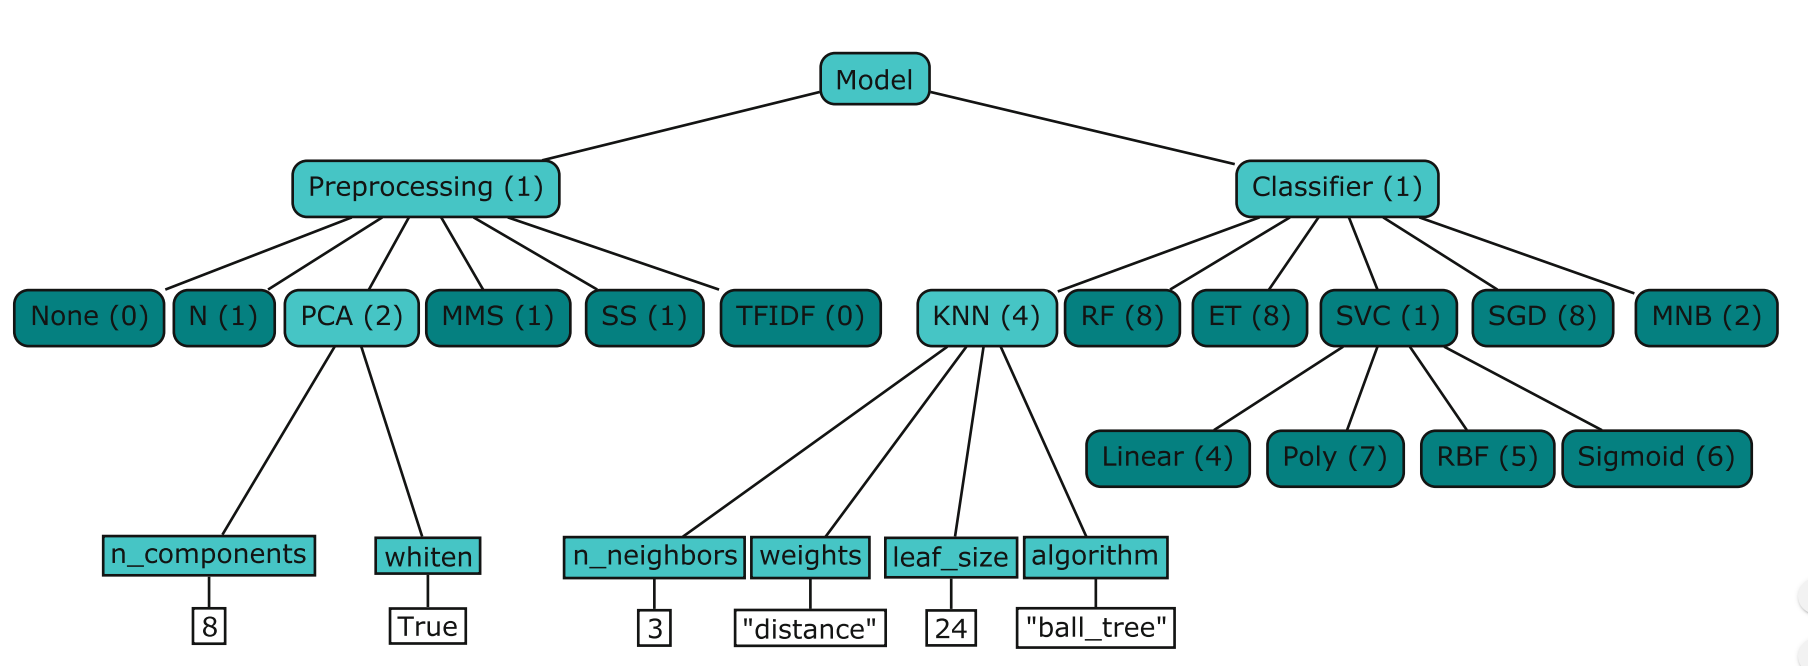
\includegraphics[width=.9\linewidth, height=0.9\textheight, keepaspectratio=true]{w06_hpo_bo/images/categ_cond_params/Conditional Parameters AutoML Book.png}
    \newline
    Example of a structured search space (Source: Figure 5.1 of the \lit{\href{https://www.automl.org/wp-content/uploads/2019/05/AutoML_Book.pdf}{AutoML book}})
\end{center}
\end{frame}
%-----------------------------------------------------------------------
\begin{frame}[c]{Categorical and Conditional Hyperparameters}
\framesubtitle{Categorical Hyperparameters}
Categorical hyperparameters are discrete hyperparameters that \emph{can not be sorted} and the \emph{distances between values might vary}. This has to be taken into account by the surrogate model:
%
\pause
%
\begin{columns}[T]
\column{0.65\textwidth}
\begin{itemize}
    \item <+-> \emph{One-hot} encoding provides a general solution
    \item <+-> Random Forests \emph{natively} handle categorical inputs
    \item <+-> Neural networks can learn \emph{entity embeddings} for categorical inputs \lit{\href{https://arxiv.org/pdf/1604.06737.pdf}{Guc et al. 2016}}
    \item <+-> Gaussian Processes can make use of the (weighted) \emph{Hamming Distance Kernel}: \lit{\href{https://www.cs.ubc.ca/~hutter/papers/Hutter09PhD.pdf}{Hutter 2009}}
\begin{equation*}
    \kernel_{\theta}(\conf_i, \conf_j) = \exp{\sum_{l=1}^d (-\theta \cdot \delta(\hyperparam_{i,l} \neq \hyperparam_{j,l}))}
\end{equation*}
\end{itemize}
%
\column{0.35\textwidth}
\vspace{0.5cm}
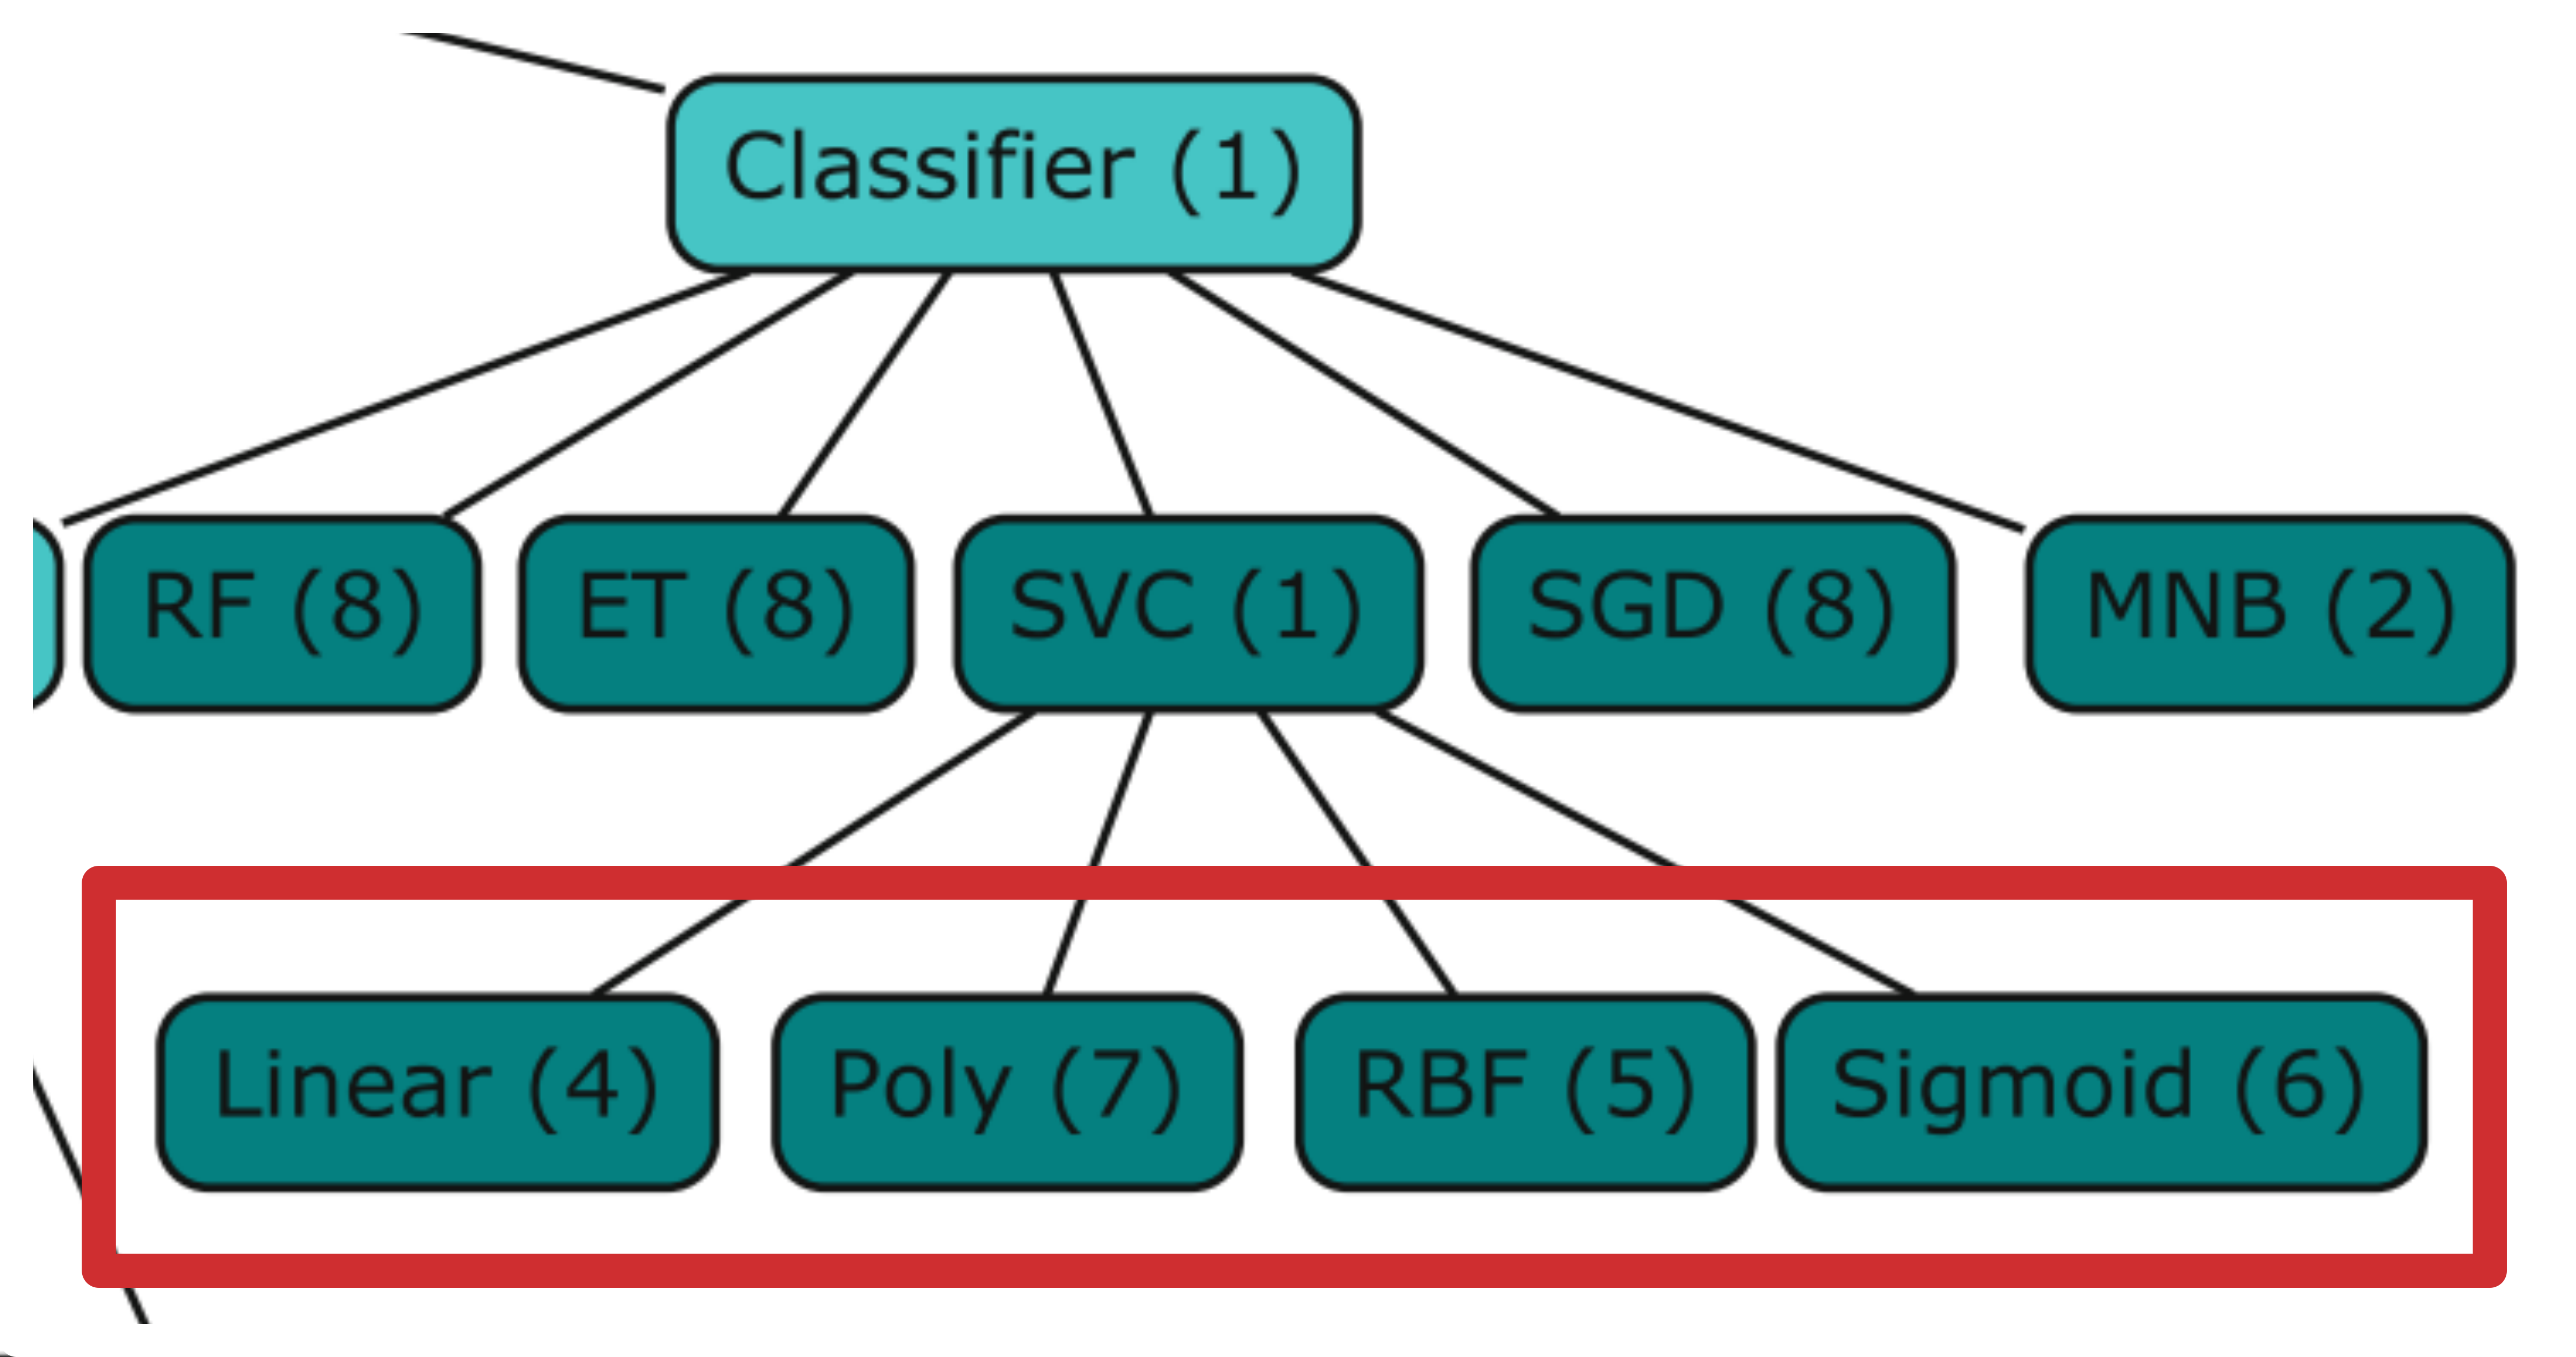
\includegraphics[width=1\textwidth]{w06_hpo_bo/images/categ_cond_params/categorical.png}
%
\end{columns}
\end{frame}
%-----------------------------------------------------------------------
\begin{frame}[c]{Categorical and Conditional Hyperparameters}
\framesubtitle{Conditional Hyperparameters}

A conditional hyperparameter is only relevant if another hyperparameter takes on a specific value and thus should be ignored by the model if not active:

\begin{columns}[T]
\column{0.65\textwidth}
 
\begin{itemize}
    \item <+-> Setting the values for inactive hyperparameter to a specific value (e.g. $0$)
    \item <+-> Random Forests \lit{\href{https://ml.informatik.uni-freiburg.de/papers/11-LION5-SMAC.pdf}{Hutter et al. 2011}} and Tree Parzen Estimators \lit{\href{http://papers.nips.cc/paper/4443-algorithms-for-hyper}{Bergstra et al. 2011}} can natively handle conditional inputs
    \item <+-> Furthermore, there exist several kernels for Gaussian Processes to handle conditional input \lit{\href{https://arxiv.org/abs/1310.5738}{Hutter et al. 2013}} \lit{\href{https://www.etsmtl.ca/Unites-de-recherche/LIVIA/Recherche-et-innovation/Publications/Publications-2017/Levesque_ijcnn_2017.pdf}{Lévesque et al. 2017}} \lit{\href{http://proceedings.mlr.press/v70/jenatton17a.html}{Jenatton et al. 2017}} 
\end{itemize}
%
\column{0.35\textwidth}
\vspace{0.5cm}
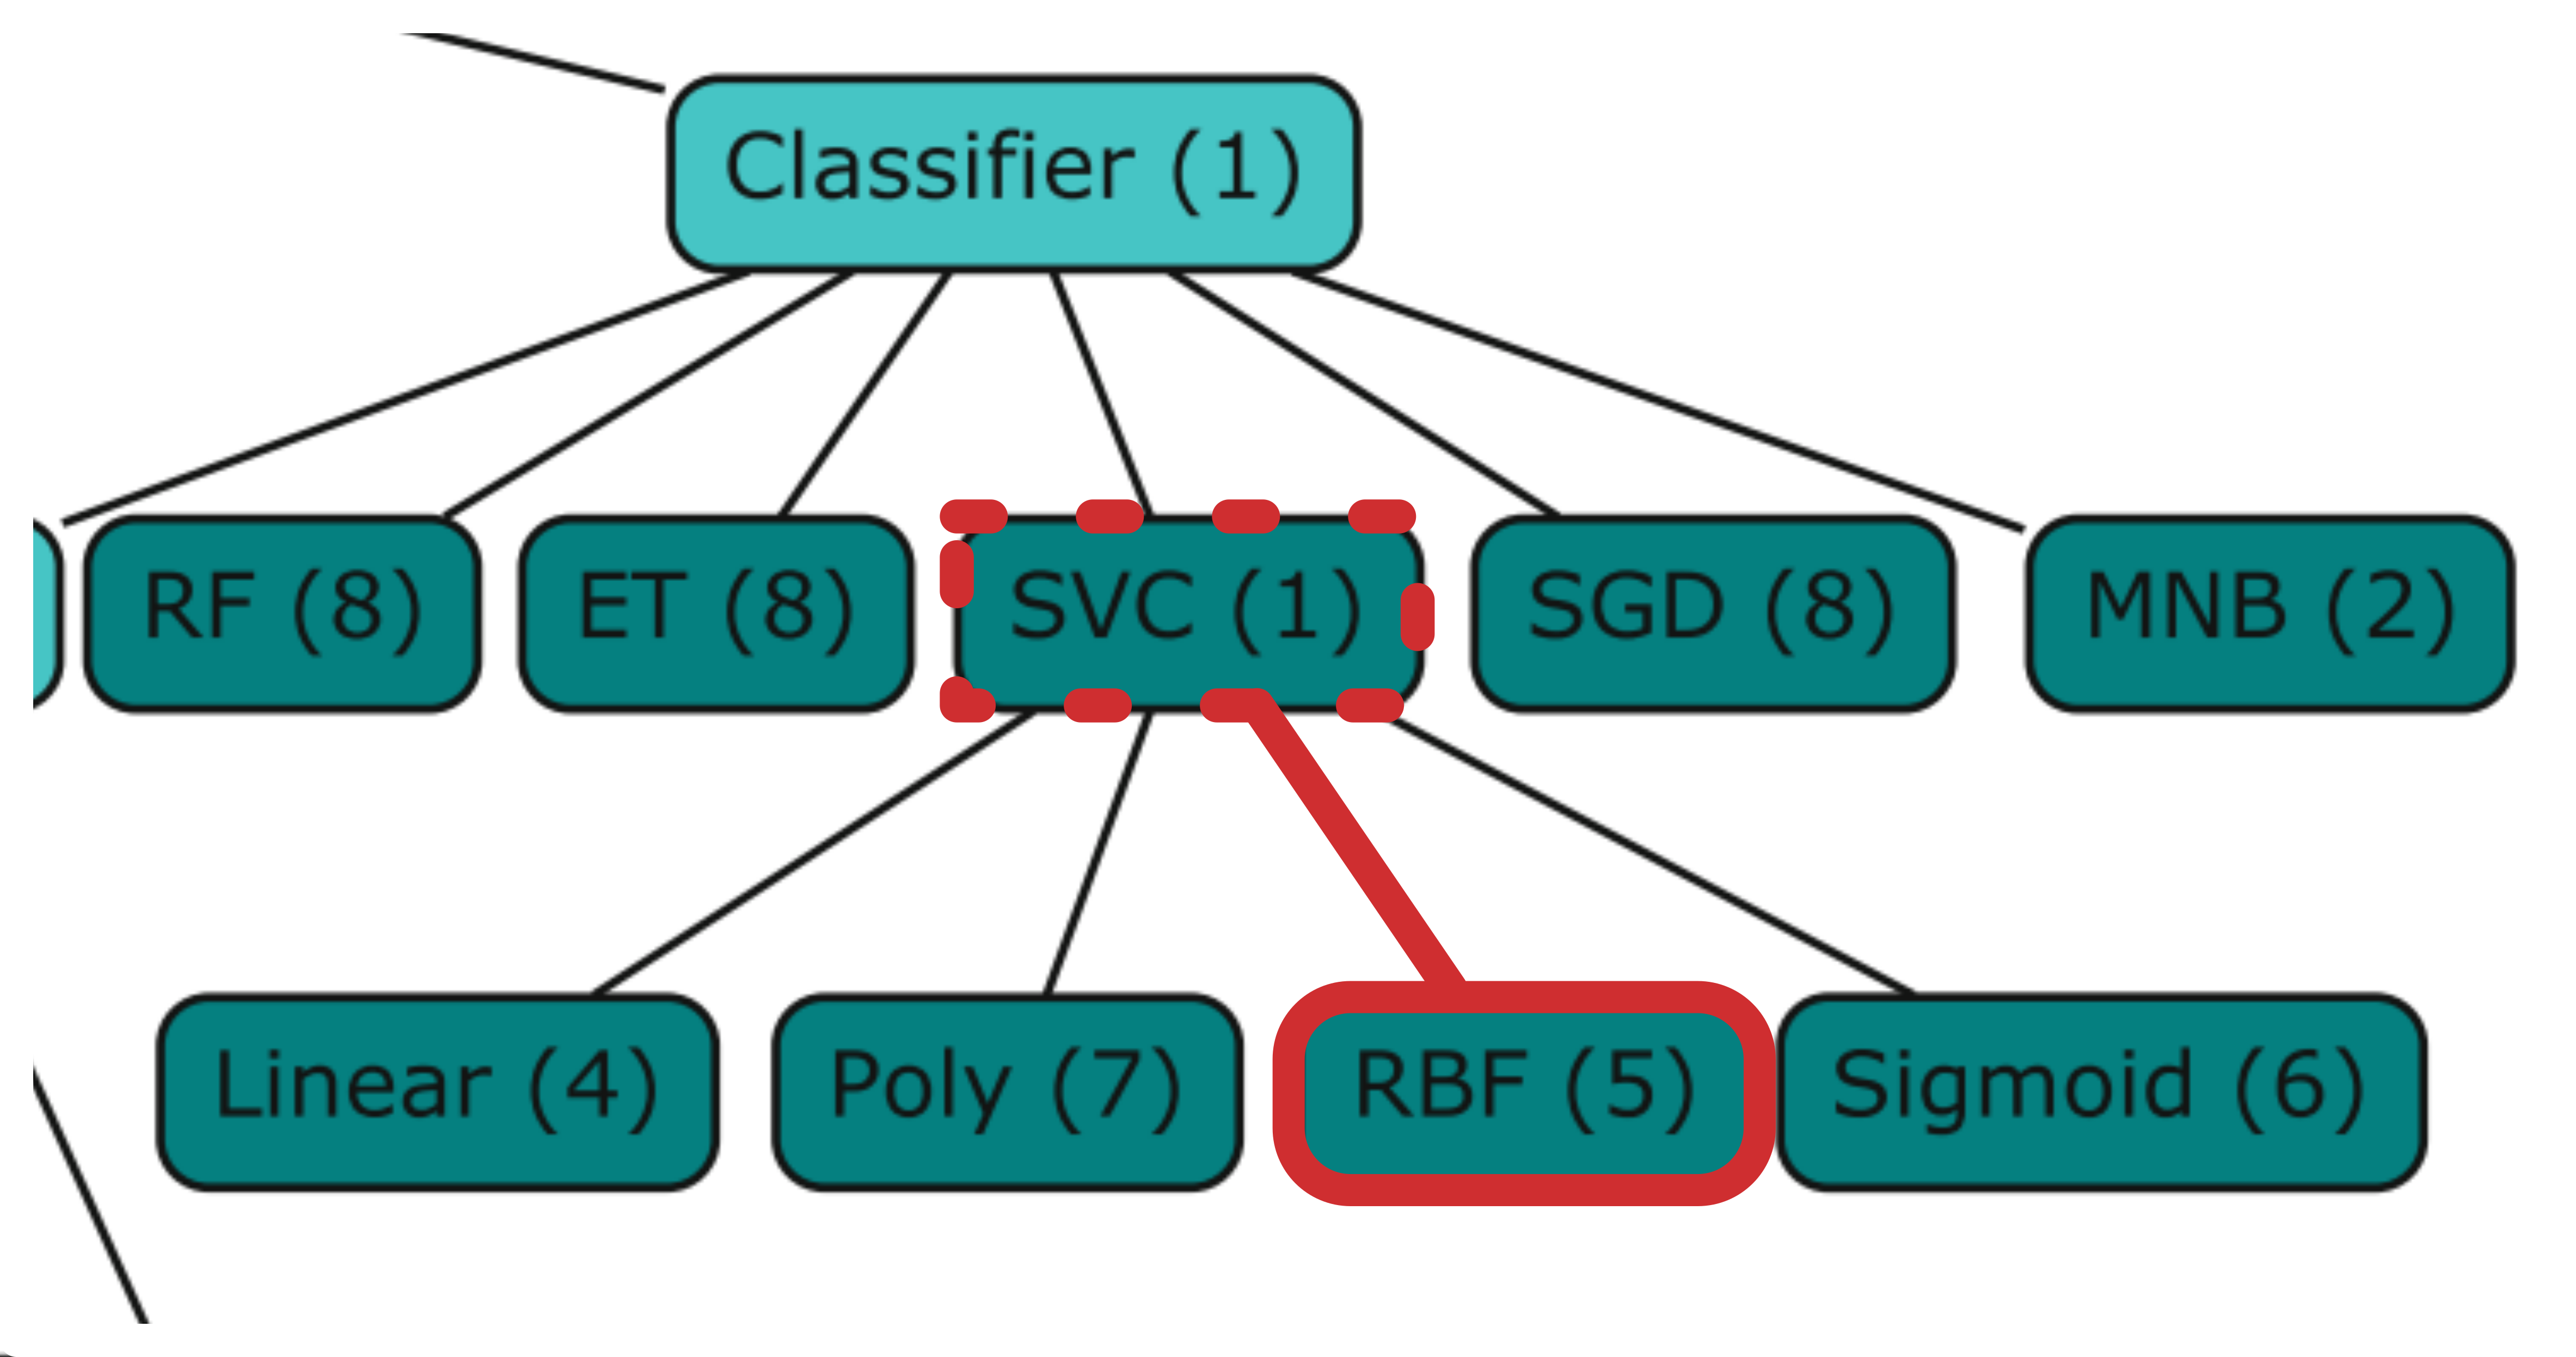
\includegraphics[width=1\textwidth]{w06_hpo_bo/images/categ_cond_params/conditional.png}
%
\end{columns}
\pause
\vspace{0.5cm}
$\xrightarrow{}$ Searching in structured search spaces is still an active research topic and is far from being solved
\end{frame}
%-----------------------------------------------------------------------
\begin{frame}[c]{High Dimensional Bayesian Optimization}
\framesubtitle{Motivation}

\begin{itemize}
%    \item Bayesian Optimization success stories:
%    \begin{itemize}
%        \item robotics, planning, recommendation, automatic algorithm configuration etc.
%    \end{itemize}
%    \pause
    \item Issue: BO works best on problems of moderate dimensions $d\leq20$
%    \pause
    \begin{itemize}
        \item Standard GPs do not tend to fit well in high dimensions
        \item Maximizing the acquisition function is also computationally challenging
    \end{itemize}
\medskip
\pause

    \item Possible solutions we will discuss:
    \begin{itemize}
        \item Embedding into a low-dimensional space (REMBO) \lit{\href{https://ml.informatik.uni-freiburg.de/papers/16-JAIR-REMBO.pdf}{Wang et al. 2016}}
        \item Additive models \lit{\href{http://proceedings.mlr.press/v37/kandasamy15.pdf}{Kandasamy et al. 2015}}
        \item Random Forests \lit{\href{https://ml.informatik.uni-freiburg.de/papers/11-LION5-SMAC.pdf}{Hutter et al. 2011}}
    \end{itemize}
\end{itemize}


\end{frame}

%----------------------------------------------------------------------

\begin{frame}[c]{High Dimensional Bayesian Optimization}
\framesubtitle{The Curse of Dimensionality vs. Low Effective Dimensionality}
\begin{itemize}
    \item Good coverage of $\pcs$ is required to ensure that the global optimum is found
    \item The number of evaluations needed to cover $\pcs$ increases exponentially with dimensionality
    \item Numerous optimization problems in practice have \emph{"low effective dimensionality"}
    \begin{itemize}
        \item E.g., HPO for neural networks and deep belief networks
        \lit{\href{http://www.jmlr.org/papers/volume13/bergstra12a/bergstra12a.pdf}{Bergstra et al. 2012}}
        \item E.g., algorithm configuration for combinatorial optimization solvers \lit{\href{http://www.jmlr.org/papers/volume13/bergstra12a/bergstra12a.pdf}{Hutter et al. 2014}}
    \end{itemize}
\pause
\medskip
    \item Idea: Exploit low effective dimensionality to cover a lower-dimensional space well
\end{itemize}

\end{frame}

%----------------------------------------------------------------------
%----------------------------------------------------------------------
\begin{frame}[c]{High Dimensional Bayesian Optimization}
\framesubtitle{Random Embeddings in a nutshell}

Given a $D=2$ dimensional black-box function $\cost(x_{1},x_{2})$:
\begin{itemize}
\begin{columns}[T]
\begin{column}{0.45\linewidth}


    \item Assume we know $\cost$ has only $d=1$ important dimensions, but we don't know which one it is.
    \end{column}
    \begin{column}{0.5\linewidth}
        \begin{figure}
    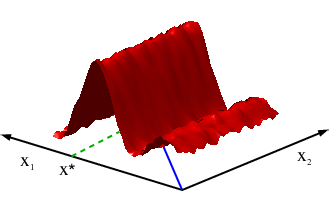
\includegraphics[width=0.5\textwidth]{images/highdim_images/Random embeddings in a nutshell1.png}
    \end{figure}
    \end{column}
\end{columns}
    \pause
    \begin{columns}[T]
    \begin{column}{0.45\linewidth}
    \vspace{-1em}
    \item Subspace $x_1=x_2$ is guaranteed to include the optimum.
        \end{column}
        \begin{column}{0.5\linewidth}
    \begin{figure}
    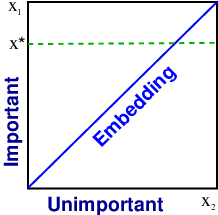
\includegraphics[width=0.5\textwidth]{images/highdim_images/Random embeddings in a nutshell2.png}
    \end{figure}
    \end{column}
\end{columns}
    \pause
\begin{columns}
\begin{column}{0.45\linewidth}
    \vspace{-8em}
    \item Idea applies to any $d$-dimensional linear subspace
    \item Allows scaling to arbitrary $D$ (e.g., $D=1$ billion)
\end{column}
\begin{column}{0.5\linewidth}

\end{column}
\end{columns}
\end{itemize}


\end{frame}

%----------------------------------------------------------------------
\begin{frame}[c]{High Dimensional Bayesian Optimization}
\framesubtitle{Random Embedding Bayesian Optimization (REMBO)}
\begin{columns}[T]
\begin{column}{0.5\textwidth}
\begin{itemize}
    \item Generate a random matrix $A \in \realnum^{D \times d}$
    \item Choose a bounded region set $\obsspace\subset\realnum^d$
    \item Use BO to optimize $g(\conf)=\cost(\pmb{Ay})$ instead of high dimensional $\cost(\conf)$
\end{itemize}
\end{column}
\begin{column}{0.5\textwidth}
\begin{figure}
    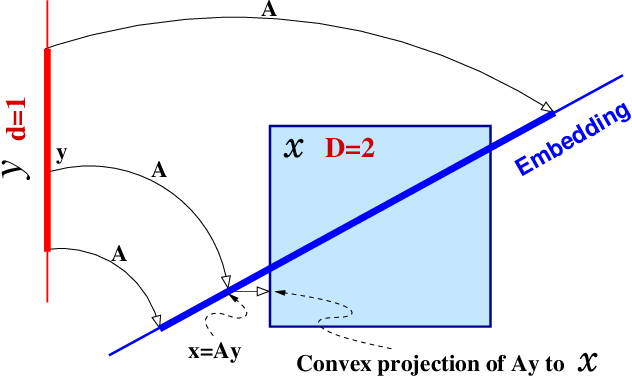
\includegraphics[width=0.8\textwidth]{images/highdim_images/Embedding.png}
\end{figure}
\end{column}

\end{columns} 
\end{frame}

%----------------------------------------------------------------------

%----------------------------------------------------------------------
\begin{frame}[c]{High Dimensional Bayesian Optimization}
\framesubtitle{REMBO- Pseudocode}


\begin{algorithm}[H]
    \SetAlgoLined
    \setcounter{AlgoLine}{0}
    \SetKwInOut{Require}{Require}
    \SetKwInOut{Result}{Result}
    
    \Require{Search space $\pcs$, cost function $\cost$, acquisition function $\acq$, predictive model $\surro$, maximal number of function evaluations $\bobudget$}
    \Result{Best observed configuration $\finconf$ according to $\iter[\bobudget]{\dataset}$ or $\surro$}
    
    \textcolor{blue}{Generate a random matrix $\pmb{A} \in \realnum^{D\times d}$}\;
    
    \textcolor{blue}{Choose the bounded region set $\obsspace\subset\realnum^d$}\;
    
    $\iter[0]{\dataset} \leftarrow \varnothing$\; 
	 
    \For{$\bocount=1$ \KwTo $\bobudget$}{
		$\iter[\bocount]{\surro} \leftarrow$ fit predictive model on $\iter[\bocount-1]{\dataset}$\;
		
		\textcolor{blue}{$\pmb{y} \leftarrow \pmb{y} \in \argmax_{\pmb{y}\in\obsspace} \acq(\pmb{y}|\iter[\bocount-1]{\dataset}, \iter[\bocount]{\surro})$}\;
		
		Query $\cost(\textcolor{blue}{\pmb{A}\pmb{y}})$;
		
		$\iter[\bocount]{\dataset} \leftarrow \iter[\bocount-1]{\dataset} \cup \{\langle \textcolor{blue}{\pmb{A}\pmb{y}}, \cost(\textcolor{blue}{\pmb{A}\pmb{y}}) \rangle \}$\;
	}
    \caption{REMBO: Bayesian Optimization with Random Embedding.}
\end{algorithm}
\end{frame}
%----------------------------------------------------------------------
\begin{frame}[c]{High Dimensional Bayesian Optimization}
\framesubtitle{Random Embedding Bayesian Optimization - Summary}
\begin{columns}[T] % align columns
\begin{column}{.48\textwidth}


    \begin{block}{Advantages}
    \begin{itemize}
    	\item Exploits low effective dimensionality 
    	\item Allows scaling to very high dimensions
    	\item Applies to both continuous and categorical variables
    	\item Trivial modification of BO algorithm
    	\item Coordinate independent (invariant under rotations)
    \end{itemize}
    \end{block}
\pause
\end{column}%

\hfill%

\begin{column}{.48\textwidth}

    \begin{block}{Disadvantages}
    \begin{itemize}
    	\item Sensitive to the definition of the bounded low dimensional constrained space $\obsspace$
    	\item Assumes truly unimportant dimensions
    	%Limits a high dimensional function in a low dimensional embedding
    	%\item Sensitive to the effective dimension
    \end{itemize}
\end{block}

\end{column}
\end{columns}   
\end{frame}

%----------------------------------------------------------------------
\begin{frame}[c]{High Dimensional Bayesian Optimization}
\framesubtitle{High Dimensional Bayesian Optimisation and Bandits via Additive Models}

\vspace{2em}
\begin{itemize}
    \item Recall:

    \begin{itemize}
        \item Standard GPs do not tend to fit well in high dimensions
        \item Maximizing the acquisition function is also computationally challenging
        \pause
    \end{itemize}
\medskip
    \item Idea:
    \begin{itemize}
        \item Assume additive structure of the objective function
        \begin{equation*}
            f(\conf)=f^{(1)}(\conf^{(1)})+f^{(2)}(\conf^{(2)})+...+f^{(M)}(\conf^{(M)})
        \end{equation*}
        \item Use an alternative acquisition function which applies to an additive kernel
    \end{itemize}
\end{itemize}

\end{frame}

%----------------------------------------------------------------------
\begin{frame}[c]{High Dimensional Bayesian Optimization}
\framesubtitle{Additive GP Models in a nutshell}
        \begin{equation*}
            f(\conf)=f^{(1)}(\conf^{(1)})+f^{(2)}(\conf^{(2)})+...+f^{(M)}(\conf^{(M)})
        \end{equation*}
\begin{itemize}
\begin{columns}[T]
\begin{column}{0.45\linewidth}

\hspace{2em}
    \item Key assumption: $f$ decomposes into lower-dimensional additive components $\conf^{(j)} \in \pcs^{(j)}, j \in \{1,..,M\}$
    \item The decompositions are disjoint $\conf^{(i)} \cap \conf^{(j)} = \varnothing$
    \pause
    \item Each decomposition $f^{(j)}(\conf^{(j)})$ is modelled by an individual GP
    \pause
    \end{column}
    \begin{column}{0.45\linewidth}
        \begin{figure}
    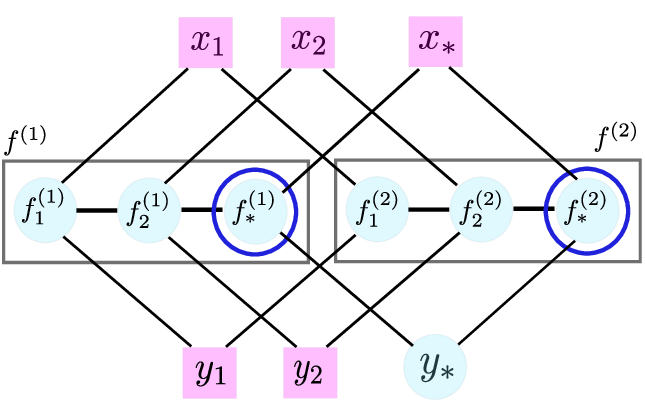
\includegraphics[width=0.7\textwidth]{images/highdim_images/additive-models.png}
    \caption{Decomposition in two additive components (M=2) \\ Source: \lit{\href{http://proceedings.mlr.press/v37/kandasamy15.pdf}{Kandasamy et al. 2015}}}
    \end{figure}
    \end{column}
\end{columns}
\end{itemize}
\end{frame}
%----------------------------------------------------------------------
\begin{frame}[c]{High Dimensional Bayesian Optimization}
\framesubtitle{Additive GP-UCB}
\begin{itemize}

    \item Idea: Represent acquisition function as sum of functions on decompositions:
    \begin{equation*}
        \acq_{t}(\conf) = \sum_{j}\acq_{t}^{(j)}(\conf^{(j)})
    \end{equation*}
\pause
\medskip    
    \item $\acq_{t}$ is maximized by maximizing each $\acq_{t}^{(j)}$ separately:
    \begin{equation*}
        \hat{\varphi}_{t}^{(j)}(\conf^{(j)}) = \mean_{t-1}^{(j)}(\conf^{(j)}) + \beta_{t}^{1/2}\stddev_{t-1}^{(j)}(\conf^{(j)})
    \end{equation*}
    \item Authors have used UCB for this work, but other acquisition functions are possible, too.
\end{itemize}
\source{\href{http://proceedings.mlr.press/v37/kandasamy15.pdf}{Kandasamy et al. 2015}}
\end{frame}
%----------------------------------------------------------------------
% \begin{frame}[c]{High Dimensional Bayesian Optimization}
% \framesubtitle{Additive GP-UCB- Pseudocode}
% \begin{algorithm}[H]
%     %\DontPrintSemicolon
%     \LinesNumbered
%     \SetAlgoLined
%     \setcounter{AlgoLine}{0}
%     \SetKwInOut{Input}{Input}
    
%     %\Input{Kernels $\kernel^{(1)},...,\kernel^{(M)}$, Decomposition $(\pcs^{(j)})_{j=1}^{M}$}\\
%     \Input{ Kernels $\kernel^{(1)},...,\kernel^{(M)}$, Decomposition $(\pcs^{(j)})_{j=1}^{M}$
%     $\dataset_{0}\leftarrow\varnothing$}
%     \For{$j=1,...,M$, $(\mean_0^{(j)},\kernel_0^{(j)})\leftarrow(0,\kernel^{(j)})$.}{
%         \For{$j=1,...,M$,}{
%             $\confI{t}_{(j)}\leftarrow\argmax_{z\in\pcs^{(j)}}\mean_{t-1}^{(j)}(z) +\sqrt{\beta_{t}}\stddev_{t-1}^{(j)}(z)$;\
            
%             $\confI{t}\leftarrow\bigcup_{j=1}^{M} \confI{t}_{(j)}$;\
            
%             $\obs\leftarrow$ Query $\cost$ at $\confI{t}$;\
            
%             $\dataset_{t}=\dataset_{t-1}\cup\{(\confI{t},\obs)\}$;\
            
%             Perform Bayesian Optimization posterior updates conditioned on $\dataset_{t}$ to obtain $\mean_{t}^{(j)},\stddev_{t}^{(j)}$ for $j=1,...,M$;\
%         }
%     }
%     \caption{Add-GP-UCB}
% \end{algorithm}
% \end{frame}


%----------------------------------------------------------------------
\begin{frame}[c]{High Dimensional Bayesian Optimization}
\framesubtitle{High dimensional BO via additive models - Summary}
\begin{columns}[T] % align columns
\begin{column}{.48\textwidth}


    \begin{block}{Advantages}
    \begin{itemize}
    	\item Exploits low effective dimensionality
    	\item Scales GP-UCB to high dimensional parameter spaces
    	\item Regret is linearly dependent on the dimension D when $\cost$ is additive
    	\item Add-GP-UCB applies to an additive kernel
    \end{itemize}
    \end{block}
\pause
\end{column}%

\hfill%

\begin{column}{.48\textwidth}

    \begin{block}{Disadvantages}
    \begin{itemize}
    	\item Relies on structural assumptions about the objective function
    	\item Restricted to an axis aligned representation
    	\item Sensitive on the number of additive components
    \end{itemize}
\end{block}

\end{column}
\end{columns}   
\end{frame}

%---------------------------------------------------------------------
\begin{frame}[c]{High Dimensional Bayesian Optimization}
\framesubtitle{Random Forests}
BO with random forests as surrogates has been shown to perform well in high dimensions:
\begin{itemize}
    \item Can handle complex parameter spaces:
    \begin{itemize}
        \item High dimensionality (low effective dimensionality)
        \item Mixed continuous/discrete parameters
        \item Conditional parameters
    \end{itemize}
\pause
\smallskip
    \item Can handle non-standard noise
    \begin{itemize}
        \item Non-Gaussian noise
        \item Heteroscedastic noise
    \end{itemize}
\pause
\smallskip
    \item Effective model for off-the-shelf Bayesian optimization
    \begin{itemize}
        \item Robustness of the model
        \item Model overhead
    \end{itemize}
\pause
\smallskip
    \item SMAC is a Bayesian optimization tool that uses random forests as a surrogate model
\end{itemize}
\end{frame}
%----------------------------------------------------------------------
\begin{frame}[c]{Parallel Bayesian Optimization}
\framesubtitle{Multi-point Acquisition Functions}

Often, there are many parallel compute resources available, but Bayesian optimization works sequentially. Extending Bayesian optimization to a parallel setting is \emph{not trivial}.
\pause
\begin{itemize}
    \item <+-> To select a batch of points in parallel we need to compute the multi-point acquisition function, e.g. Expected Improvement:
    \begin{equation*}
        q\text{-EI}(\conf_{1, \dots, q}) = \E \left[ \cost(\incumbent) - \min_{i=1, \dots, q} \surro(\conf_i) \right]
    \end{equation*}
    \item <+-> For EI and KG, this requires \emph{expensive-to-compute} q-dimensional Gaussian cumulative distributions and is thus also \emph{expensive to maximize}. \lit{\href{https://hal.archives-ouvertes.fr/hal-00260579/document}{Ginsbourger et al. 2007}}, \lit{\href{https://arxiv.org/pdf/1606.04414v4.pdf}{Wu et al. 2018}}, \lit{\href{https://arxiv.org/abs/1805.10196}{Wilson et al. 2018}}, \lit{\href{https://arxiv.org/pdf/1602.05149.pdf}{Wang et al. 2019}}
\end{itemize}
\pause
\end{frame}
%----------------------------------------------------------------------
\begin{frame}[c]{Parallel Bayesian Optimization}
\framesubtitle{Constant Liar, Kriging Believer and Fantasies}
Assume we do not want to select a batch of points, but to choose the next $\conf$ while there are still \emph{pending evaluations}. 
\pause
%
A conceptually simple method is to assume observations for the outstanding evaluations and perform sequential optimization:
\pause
\begin{itemize}
    \item <+-> \emph{Constant Liar}: Choose a fixed value (constant) \lit{\href{http://www.cs.ubc.ca/labs/beta/EARG/stack/2010_CI_Ginsbourger-ParallelKriging.pdf}{Ginsbourger et al. 2010}}
    \item <+-> \emph{Kriging Believer}: Use the current mean prediction (belief)  \lit{\href{http://www.cs.ubc.ca/labs/beta/EARG/stack/2010_CI_Ginsbourger-ParallelKriging.pdf}{Ginsbourger et al. 2010}}
    \item <+-> \emph{Fantasies}: Use Monte Carlo estimates (fantasies, more details on the next slide).
\end{itemize}
\end{frame}
%----------------------------------------------------------------------
\begin{frame}[c]{Parallel Bayesian Optimization}
\framesubtitle{Constant Liar, Kriging Believer and Fantasies}
%
Assume we have observed data $\left\{ \left\langle \bonextsample, \bonextobs \right\rangle \right\}^{N}_{\bocount = 1}$ and $J$ evaluations are pending $\left \{\conf_{j} \right \}^{J}_{j = 1}$. We can compute the expected mean function using the following integral: \pause
\begin{equation*}
\begin{aligned}
    \Bar{\acq} \left( \conf; \left\{ \left\langle \bonextsample, \bonextobs \right\rangle \right\}^{N}_{\bocount = 1}, \left \{\conf_{j} \right \}^{J}_{j = 1} \right) =  \pause
    \int_{\mathbb{R}^J}  \acq \left( \conf; \left\{ \left\langle \bonextsample, \bonextobs \right\rangle \right\}^{N}_{\bocount = 1}, \left \{ \left\langle \conf_j, \obs_j \right\rangle \right \}^{J}_{j=1} \right) \\
    p( \{ \obs_j \}^{J}_{j = 1}  \rvert \{ \conf_j \}^{J}_{j = 1}, \left \left\{ \left\langle \bonextsample, \bonextobs \right\rangle \right\}^{N}_{\bocount = 1} )d\obs_1 \dots d\obs_J
\end{aligned}
\end{equation*}
%
\vspace{-0.8cm}
\begin{columns}
\column{0.6\textwidth}
\only<4->{
\begin{enumerate}
    \only<4->{\item Evaluated observations: $\left \{\conf_1, \conf_3, \conf_4 \right \}$, pending: $\left \{\conf_2, \conf_5 \right \}$.}
    \only<5->{\item Fit a model for each possible realization of $\left \{\cost(\conf_2), \cost(\conf_5) \right \}$.}
    \only<6->{\item Calculate acquisition function for each model.}
    \only<7->{\item Integrate all acquisition functions over $\conf$.}
\end{enumerate}
}

\column{0.4\textwidth}
    \only<4-5>{
    \begin{figure}
        \centering
        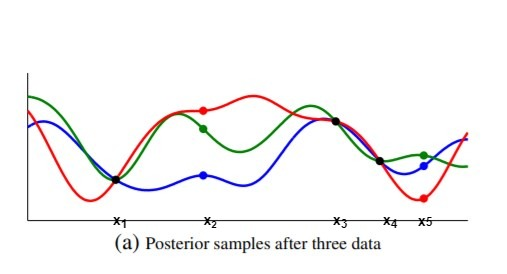
\includegraphics[width=0.8\textwidth]{w06_hpo_bo/images/parallel/parallel_a.jpg}
    \end{figure}
    }
    \only<6>{
    \begin{figure}
        \centering
        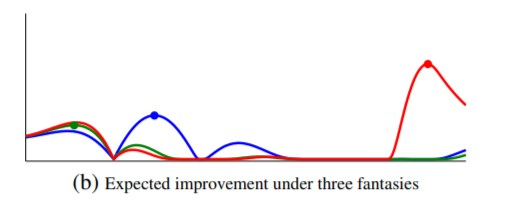
\includegraphics[width=0.8\textwidth]{w06_hpo_bo/images/parallel/parallel_b.jpg}
    \end{figure}
    }
    \only<7->{
    \begin{figure}
        \centering
        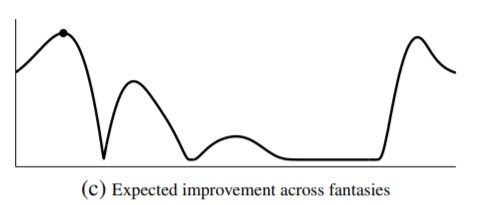
\includegraphics[width=0.8\textwidth]{w06_hpo_bo/images/parallel/parallel_c.jpg}
    \end{figure}
    }
\end{columns}

\source{\href{https://papers.nips.cc/paper/4522-practical-bayesian-optimization-of-machine-learning-algorithms.pdf}{Snoek et al. 2012}}

\end{frame}
%
%\begin{frame}
%\begin{itemize}
%    \item <+-> Utilize tractable properties of GP to get Monte Carlo estimates of %acquisition function under different results from pending function evaluations. \pause
%    \item <+-> Consider the case where $N$ evaluations have completed, with data $\left \{\bonextsample, \bonextobs \right \}^{N}_{\bocount = 1}$ and $J$ evaluations are pending $\left \{\conf_{j} \right \}^{J}_{j = 1}$: \pause
%    \begin{equation*}
%        \begin{aligned}
%            \hat{\acq} ( \conf; \left \{ \bonextsample, \bonextobs \right \}, \left \{ \conf_j \right \} ) =  \pause
%            \int_{\mathbb{R}^J}  \pause \acq ( \conf; \left \{ \bonextsample, %\bonextobs \right \}, \left \{ \conf_j, \obs_j \right \} ) \\  \pause
%            p(\left \{ \obs_j \right \}^{J}_{j = 1}  \rvert \left \{ \conf_j \right \}^{J}_{j = 1}, \left \{ \bonextsample, \bonextobs \right \}^{N}_{\bocount=1} )d\obs_1 \dots d\obs_J
%        \end{aligned}
%    \end{equation*}
%\end{itemize}

%\source{\href{https://csc2541-f17.github.io/}{Scalable and Flexible Models of Uncertainty, University of Toronto}}

%\end{frame}
%-----------------------------------------------------------------------
\begin{frame}[c]{Further extensions}
\framesubtitle{Noisy Evaluations}

\small

\begin{columns}[T]

    \column{0.6\textwidth}

    \begin{itemize}
        \item Given noisy evaluations, GP regression proceeds similarly to the noiseless case by adding the variance to the diagonal of the covariance matrix.
        \vspace{-0.2cm}
        \item KG and ES directly handle noisy function evaluations~\lit{\href{https://arxiv.org/abs/1807.02811}{Frazier 2018}}.
        \vspace{-0.2cm}
        \item Computing EI with observation noise is challenging:
        \vspace{-0.2cm}
        \begin{itemize}
            \item Uncertainty about which point is the current incumbent $\incumbent[\bocount-1]$.
            \item Uncertainty about the costs $\cost(\conf_i)$.
        \end{itemize}
    \end{itemize}
    
    \column{0.4\textwidth}
    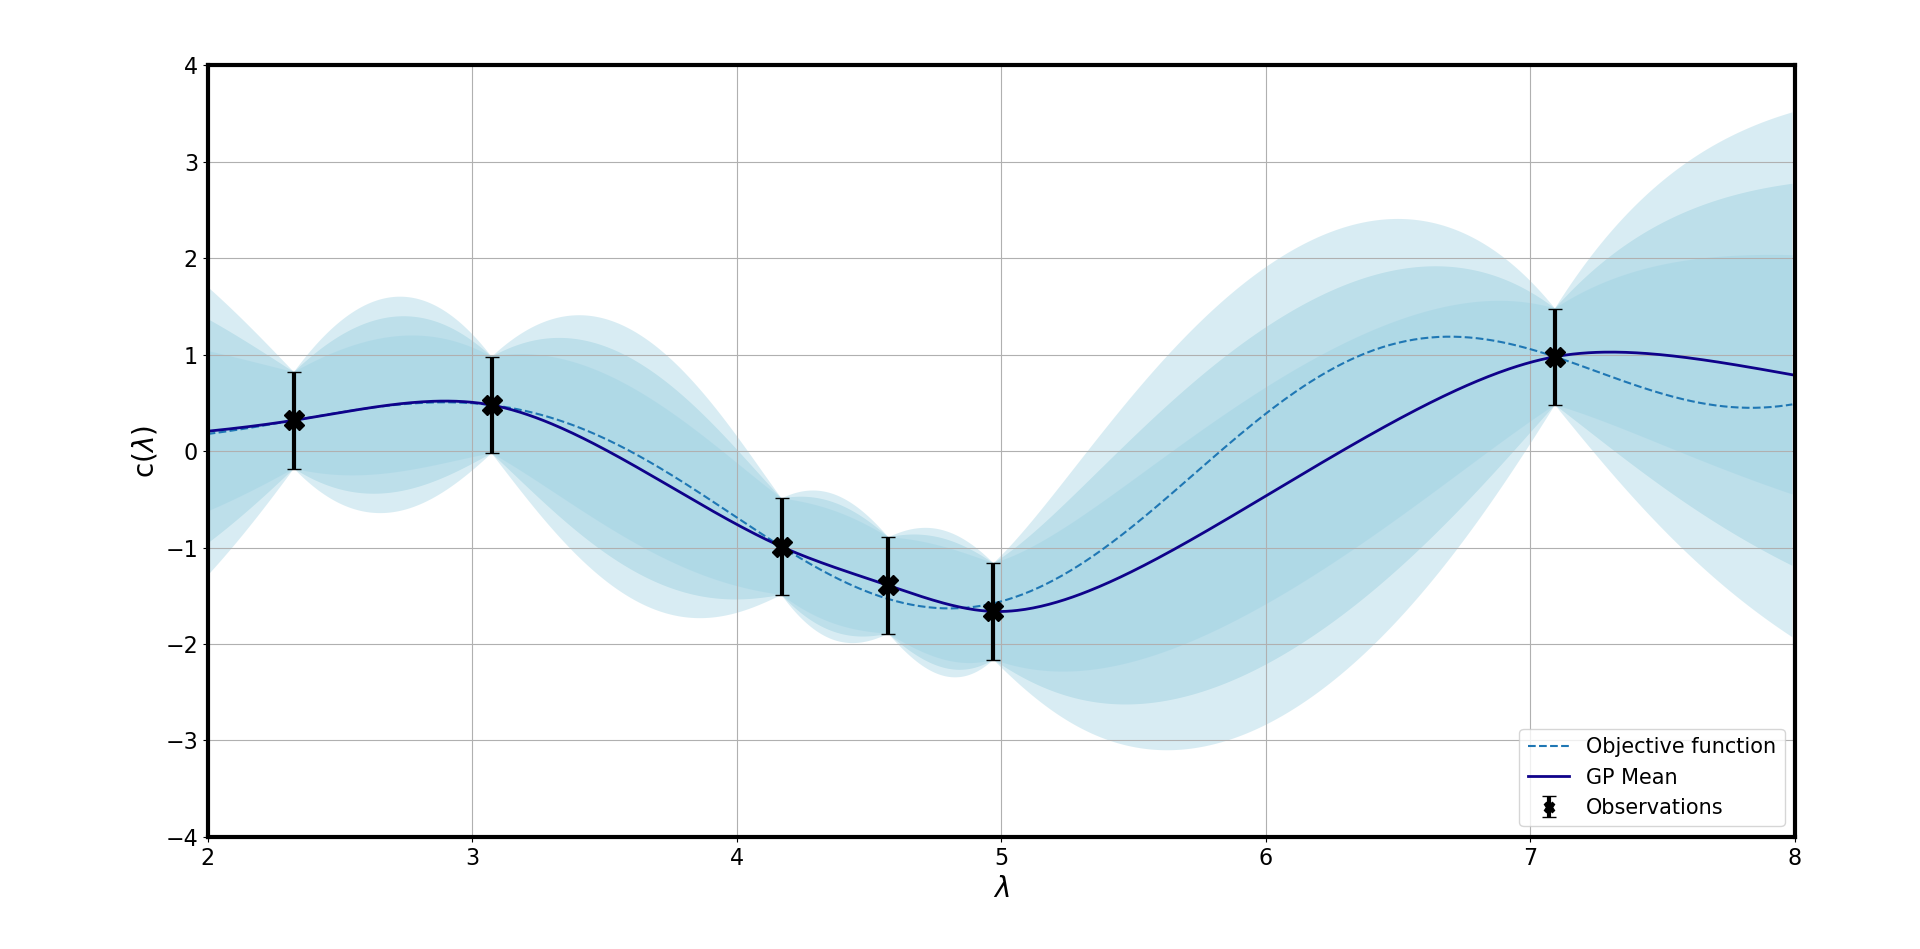
\includegraphics[width=\textwidth]{images/extensions/BO_Loop_Noisy3.png}
    
\end{columns}
\begin{itemize}
    \item Noisy Expected Improvement~\lit{\href{https://arxiv.org/abs/1706.07094}{Letham et al. 2019}} extends the regular Expected Improvement by integrating over the predictive posterior of the model:
    % There's an additional paper by Gramacy and Lee from 2011 which does a more complicated treatment of noise in EI
    \begin{equation*}
        \acq_{NEI}(\conf|\dataset)=\int_{\surro}\acq_{EI}(\conf|\surro)p(\surro|\dataset)\text{d}\surro
    \end{equation*}
    \vspace{-0.2cm}
    \begin{itemize}
        \item Compute with Monte Carlo Integration.
        \item Each sample from the model posterior has its own incumbent $\incumbent[\bocount-1]$.
    \end{itemize}
    \end{itemize}
\end{frame}

%----------------------------------------------------------------------

\begin{frame}[c]{Further extensions}
\framesubtitle{Constrained Bayesian Optimization}

\begin{columns}[T]

\column{0.6\textwidth}

Four types of constraints
\begin{small}
\begin{enumerate}
    \item Known constraints: can be accounted for when optimizing $\acq$
    %\item Policy constraints: function value is observed, but deemed forbidden~\lit{\href{https://www.soe.ucsc.edu/sites/default/files/technical-reports/UCSC-SOE-10-10.pdf}{Lee and Gramacy 2010}}
    \item Hidden constraints: no function value is observed due to a failed function evaluation~\lit{\href{https://www.soe.ucsc.edu/sites/default/files/technical-reports/UCSC-SOE-10-10.pdf}{Lee and Gramacy 2010}}
    \item Unknown constraints: there's an additional, but unknown constraint function, for example the memory used, which can be observed and modeled
\end{enumerate}
\end{small}

\column{0.4\textwidth}
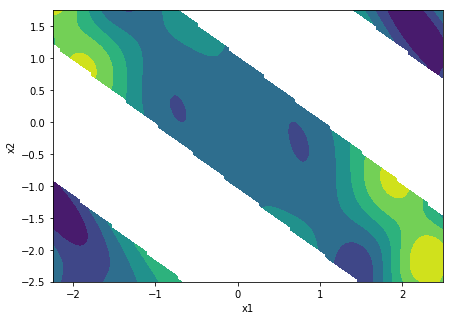
\includegraphics[width=0.9\textwidth]{images/extensions/notebooks_constrained_bo_4_0.png}\\
	\footnotesize{Hidden constraints. Image source: \lit{\href{https://gpflowopt.readthedocs.io/en/latest/notebooks/constrained_bo.html}{GPFlowOpt Tutorial, Apache 2 License}}}

\end{columns}

Most general solution: \emph{Expected Constrained Improvement}~\lit{\href{https://www.soe.ucsc.edu/sites/default/files/technical-reports/UCSC-SOE-10-10.pdf}{Lee and Gramacy 2010}}:
\vspace{-0.1cm}
\begin{equation}
    ECI(\conf) = EI(\conf)h(\conf),
\end{equation}
\vspace{-0.1cm}
where $h(\conf)$ is the probability that $\conf$ is a valid configuration.

\vspace{0.1cm}
Further literature in \lit{\href{https://arxiv.org/abs/1807.02811}{Frazier 2018}} and \lit{\href{https://link.springer.com/chapter/10.1007/978-3-030-05318-5_1}{Feurer and Hutter 2019}}.

\end{frame}
%----------------------------------------------------------------------
\begin{frame}[c]{Further extensions}
\framesubtitle{Even more extensions}
Bayesian optimization has been extended to numerous scenarios:
\begin{itemize}
    \item Multi-task, Multi-fidelity and Meta-learning $\rightarrow$ separate lecture
    \item Multi-objective Bayesian optimization $\rightarrow$ separate lecture
    \item Bayesian optimization with safety guarantees~\lit{\href{http://proceedings.mlr.press/v37/sui15.pdf}{Sui et al. 2015}}
    \item Directly optimizing for ensemble performance~\lit{\href{http://auai.org/uai2016/proceedings/papers/73.pdf}{Lévesque et al. 2016}}
    \item Combination with local search methods~\lit{\href{https://www.researchgate.net/publication/241216681_Bayesian_Guided_Pattern_Search_for_Robust_Local_Optimization}{Taddy et al. 2009}}
    \item Can optimize anything that can be described by a kernel, such as neural network architectures~\lit{\href{https://papers.nips.cc/paper/7472-neural-architecture-search-with-bayesian-optimisation-and-optimal-transport.pdf}{Kandasamy et al. 2018}} or a latent embedding, such as molecules~\lit{\href{https://arxiv.org/abs/1709.05501}{Griffiths et al. 2017}}
    \item Many more, too many to mention
\end{itemize}
  
\end{frame}
%-----------------------------------------------------------------------
\begin{frame}[c]{Questions to Answer for Yourself / Discuss with Friends}

\begin{itemize}
% Categorical and Conditional
\item \emph{Discussion.} What would happen if you treat a categorical hyperparameter as a continuous hyperparameter, e.g. ${0, 0.5, 1}$ instead of ${A, B, C}$, in Bayesian optimization using a Gaussian Process?
\item \emph{Repetition.} What is the main idea behind additive modelling? Is this assumption realistic?
% Parallel
\item \emph{Repetition.} Which method can you use to impute values for outstanding evaluations. What are advantages and disadvantages of each method?
% Noise & Constrained
\item \emph{Discussion.} What are worst case scenarios that could happen if you ignore the noise during Bayesian optimization?
% Further
\end{itemize}
\end{frame}